\paragraph*{Configurable Systems} Modern software systems usually need to be
customized to specific customer needs. Customizable software, for instance, enables greater
flexibility in supporting variable platforms to be run on or to tweak
performance. Customization is realized by providing a configurable software
that ships with a variety of \emph{configuration options}, or \emph{features} to
select from \citep{apel_feature-oriented_2013}.
Options  can range from fine-grained options that tune small functional- and
non-functional aspects to those that enable or disable entire subsystems of the
software. Examples for configurable software systems range from small
open-source command line tools to mature platforms like Eclipse or even entire
operating systems like the Linux kernel with more than $11.000$ options
\citep{dietrich_robust_2012}.

The design and development of configurable software systems is divided into
\emph{problem space} and \emph{solution space} \citep{czarnecki_generative_2000}. The problem space
comprises the abstract design of features that are contained in the software system as well as
constraints among features, such as dependencies or mutual-exclusion. The
solution space describes the technical realization of features and the
functionality described by and associated with features (e.g., implementation
and build mechanism). That is, features are mapped to corresponding code
artifacts and, hence, cross both spaces.

A common way to express features and constraints in the problem space is to
define a \emph{variability model}, or \emph{feature model} which subsumes all
valid configurations \citep{apel_feature-oriented_2013}. There are different and equivalent syntactical
approaches to define feature models, for instance, a propositional formula $F$ over the set of
features of the configurable software systems \citep{batory_feature_2005}. In
this case a configuration is valid with respect to the feature model if and only if $F$ holds for all
selected features being true and all unselected features being false respectively. 
However, a more practical and more commonly used way to express feature models
are graphical tree-like \emph{feature diagrams}
\citep{apel_feature-oriented_2013}. In a feature diagram, features are ordered
hierarchically, starting with a root feature and subsequent child features. By
definition, the selection of a child feature requires the parent feature to be
selected as well. Child features can either be labeled as \emph{optional}
features  or \emph{mandatory} features; the latter ones need to be selected in
every valid configuration.
Moreover, feature diagrams
provide a syntax for two different types of feature groups, \emph{or-groups} or
\emph{alternative-groups}. In an or-group, at least one of the group's features
needs to be selected for a valid configuration, whereas in an alternative group
exactly one out of the group's mutually exclusive features must be selected. In
addition to the feature hierarchy, constraints, which cannot be expressed by
the tree-like structure, are referred to as \emph{cross-tree constraints} and
are depicted by arrows between two features. For such two features $f_1$ and $f_2$,
a cross-tree constraint means that for feature $f_1$ to be selected,  either the
selection of $f_2$ is required/implied or excluded.

An introductory example for the syntax and semantics of feature diagrams is
provided in Fig.~\ref{fig:introduction_fm}. In this example, for an imaginary
vehicle propulsion can be configured with eight valid configurations. The vehicle requires an engine,
thus, feature \textsf{Engine} is mandatory. At least one out of the three
features \textsf{Hybrid}, \textsf{Piston} and \textsf{Electric} needs to be
selected. For a piston engine, we can select either the feature \textsf{Diesel}
or \textsf{Petrol}. A petrol engine requires additional ignition sparks in
contrast to a Diesel engine. For an electric engine a battery we require a
battery, hence, the feature \textsf{Battery} is mandatory.
In addition, the feature model specifies two cross-tree constraints: First, the
feature \textsf{Tank} is optional, yet once a piston engine is selected, we
require  a tank. Second, since we want to use the Hybrid functionality (e.g.,
use both electric and piston engine simultaneously), we require to have both a piston
and an electric engine to be selected.

\begin{figure}[htbp]
  \centering
  	
  	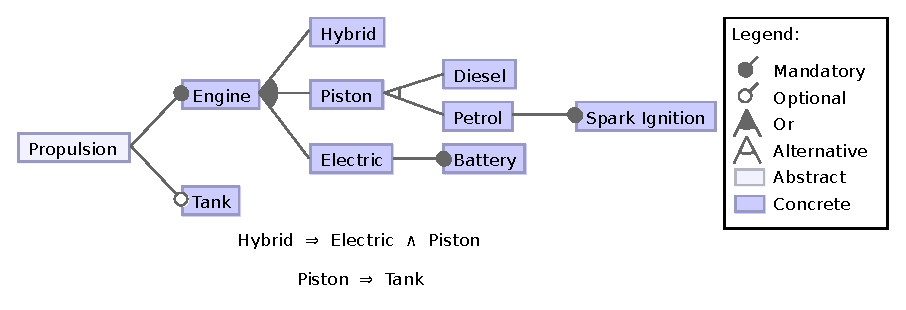
\includegraphics[width=0.85\textwidth]{images/introduction_fm.eps}
  \caption{Feature diagram for a feature model with eight valid configurations;
  two cross-tree constraints are specified as propositional formulas over
  features}
  \label{fig:introduction_fm}
\end{figure}

For a configurable system configurations are primarily chosen to meet
functional and/or non-functional requirements. Nonetheless, the selection of
certain combinations of multiple features, of course, can happen to cause
unexpected and undesired side effects as well. This so-called \emph{feature
interaction} is an ``emergent behavior that cannot be easily deduced from the
behaviors associated with the individual features involved''
\citep{apel_feature-oriented_2013} and can make development and
maintenance of a configurable system an error prone task. 
A commonly referred to example of a feature interaction, as drafted by
\cite{calder_feature_2003}, describes interactions in telecommunication networks. Given two
independent features \textsf{CallForwarding} and \textsf{CallWaiting}, where \textsf{CallForwarding} forwards a call from a busy line to a line that is
available, and where \textsf{CallWaiting} notifies a busy line when a call is on
hold. In isolation their behavior is well-defined, but if both features are selected their oppositional
behavior becomes problematic. If no precedence of one feature has been
specified, the network might end up in race conditions or other unexpected
behavior. That is, to avoid this feature interaction, for instance, precedence
constraints must be implemented or the selection of both features must be
mutually exclusive.


\paragraph*{Thesis Statement and Scope}
A software system’s performance depends on the functionality offered, the
respective implementation, program load and the resulting execution. While
feature interactions not necessarily cause the software system to break
severely in all cases, its overall performance can degrade for corner cases or
specific configurations as the feature selection influences the execution. That
is, the choice of features as well shapes the performance of a software system.

Configuration options for software systems are usually constrained (e.g., are
mutually exclusive, imply or depend on other features) to a certain extent. In
the worst case though, where all options can be selected independently, the
number of valid configurations grows exponentially with every feature added and
likely exceeds the number of atoms in the entire universe once we count $265$
independent features. Hence, even for a small number of features, any naive
approach to assessing properties of configurable software systems exhaustively
for each valid configuration is in general conceived infeasible. Despite this
mathematical limitation, many feasible approaches to static analysis for highly
configurable systems emerged. Those variability-aware approaches enable , for
instance, {\color{gray} type checking etc} in the presence of variability by
exploiting commonalities among different variants \citep{thum_classification_2014}.

The aspect of performance of configurable software systems has gained more
attention recently, even though from a practitioners view, according to
\cite{molyneaux_art_2014}, for the most part performance testing is still not
accommodated to an acceptable degree in the development process.
Assessing performance for configurable systems incorporates obtaining knowledge about the performance of
every valid configuration. In the recent past, the a variety of approaches to
model, learn and predict performance behavior for configurable software system
have emerged. The scheme behind these approaches is the conception of
performance modeling as an optimization problem, i.e., to recover and
approximate performance behavior and respective dependencies from the selection
of configuration options.

Genetic algorithms \citep{guo_genetic_2011,sayyad_scalable_2013}  have shown
reasonable results, yet are not able to handle constraints like mutual
exclusion. In 2012 \citeauthor{siegmund_predicting_2012} proposed a
method to predict performance for arbitrary variants following an approach for
automated detection of feature interaction \citep{siegmund_predicting_2012}.
Following their approach, in 2015 they proposed performance-influence models as a means
to analyze and predict performance for configurable software systems
\citep{siegmund_performance-influence_2015}. A performance-influence model
attempts to approximate the influence of both single features and interacting
features on the software systems' performance.
The approach has shown a reasonably low error rate for several real-world
applications and allows prediction of system performance for arbitrary
configuration variants.

Going a step further, actively maintained configurable software systems, of
course, evolve: Variability models might change as software has to adapt to
changes in the functional requirements it is meant to meet. Patching and
upgrading a software system affects the architecture or implementation that is
likely to become inconsistent and degrade over time. While there exists
substantial work on understanding the evolution of configurable systems, e.g.,
documenting common symptoms of architectural decay \citep{passos_feature_2015,zhang_variability_2013} or
attempting to classify patterns for variability evolution
\citep{seidl_co-evolution_2012,peng_analyzing_2011,passos_towards_2012}, there
is little we know so far about the evolution of performance or non-functional
properties in configurable systems.

We believe that to get a better understanding software evolution and to address
performance regression problems it is inevitable to continue studying the
performance and performance evolution of configurable systems. In practice, all
aforementioned approaches to model and predict performance behavior for a
configurable software system require exhaustive records of performance
measurements to learn from. Even though valid configurations can be sampled to
some extent \citep{apel_feature-oriented_2013}, assessing a single version of a configurable software
system still demands a large number of valid configurations to be measured. In
addition, to study the performance evolution of configurable software systems a
history or series of performance models is required. That is, assessing
performance evolution of configurable systems is infeasible without tool
support.\\

The goal of this thesis is to provide a theoretical and practical foundation for
exhaustive performance measurements of configurable software systems and series
thereof. We contribute a guideline of and tool support for performance
measurements in the presence of variable and evolving software. Our research
objectives and desired outcomes are

\begin{itemize}
  \item a survey of the phenomenon of performance evolution and corresponding
  best practices in performance testing, strategies to address configuration space explosion and 
  \item an automated tool support for performance measurement for multiple
  revisions of configurable software systems.
\end{itemize}

\paragraph*{Thesis Outline}
The Thesis is organized as follows. Chapter \ref{chapter:2} recalls the background
topics of the thesis theme, including software evolution, the foundations and statistical
aspects of performance testing, variability model synthesis, and recent
approaches to performance modeling. In Chapter \ref{chapter:3} we present the
overall measurement process and discuss the methods used for our performance
measurement tool as well as its limitations. In Chapter \ref{chapter:4} we evaluate practical
aspects of our tool with respect to practicality and discuss the results
thereof. Finally, Chapter \ref{chapter:5} concludes the thesis and gives an
outlook on possible future work.
